\chapter{Results}
This results chapter is meant as a mechanism to present all of the data that was collected on the performance of different demodulator. All of the demodulators that were tested in the course of this research will be shown whether that be dedicated hardware or software. The first results that will be shows are those of the dedicated hardware, being TNCs and Argent Data's Open Trackers. Following the hardware will be the software implementations. And following that will be some general comparisons between the hardware and software.

\section{Dedicated Hardware Results}
Before presenting all of the data on how many packets were correctly demodulated in each one of the five test files, each one of the pieces of hardware will listed.  In the scope of this research a total of 12 pieces of hardware were tested and they are Argent Data's Open Tracker 2, Open Tracker 3, Open Tracker USB, Open Tracker 3 Micro, Kantronics Kam, two Kantronics Kam Plus, two AEA PK-88, a PK-232, a PK-232MBX, and an MFJ-1278. Please note that on the figures Open Tracker will be abbreviated OT.

The first two tests consisting of clean packets - 40 generated from the Open Tracker and 200 using Toledo's suite - was relatively uninteresting. Essentially every piece of hardware decoded all 40 and all 200 packets. The only anomalies to this were that the Open Tracker USB was only able to decode 39 and 193 out of the 40 and 200 packet files respectively. Additionally the Open Tracker 3 Micro missed one packet in the 200 packet file to only decode 199. For these since there is no real way to debug and see the cause of decoding relatively fewer or more packets just the data is presented as it was measured to allow for comparison to the software. This will continue to be the case for the remainder of this hardware section.

Following the two easy files the next file is same content as the file with 40 packets in it with the only difference being that noise was progressively added. In Figure \ref{allHardwareOT3Noise} the two PK-88s stand out for being able to decode 25 of the 40 packets in this file.

 \begin{figure}
  \centering
	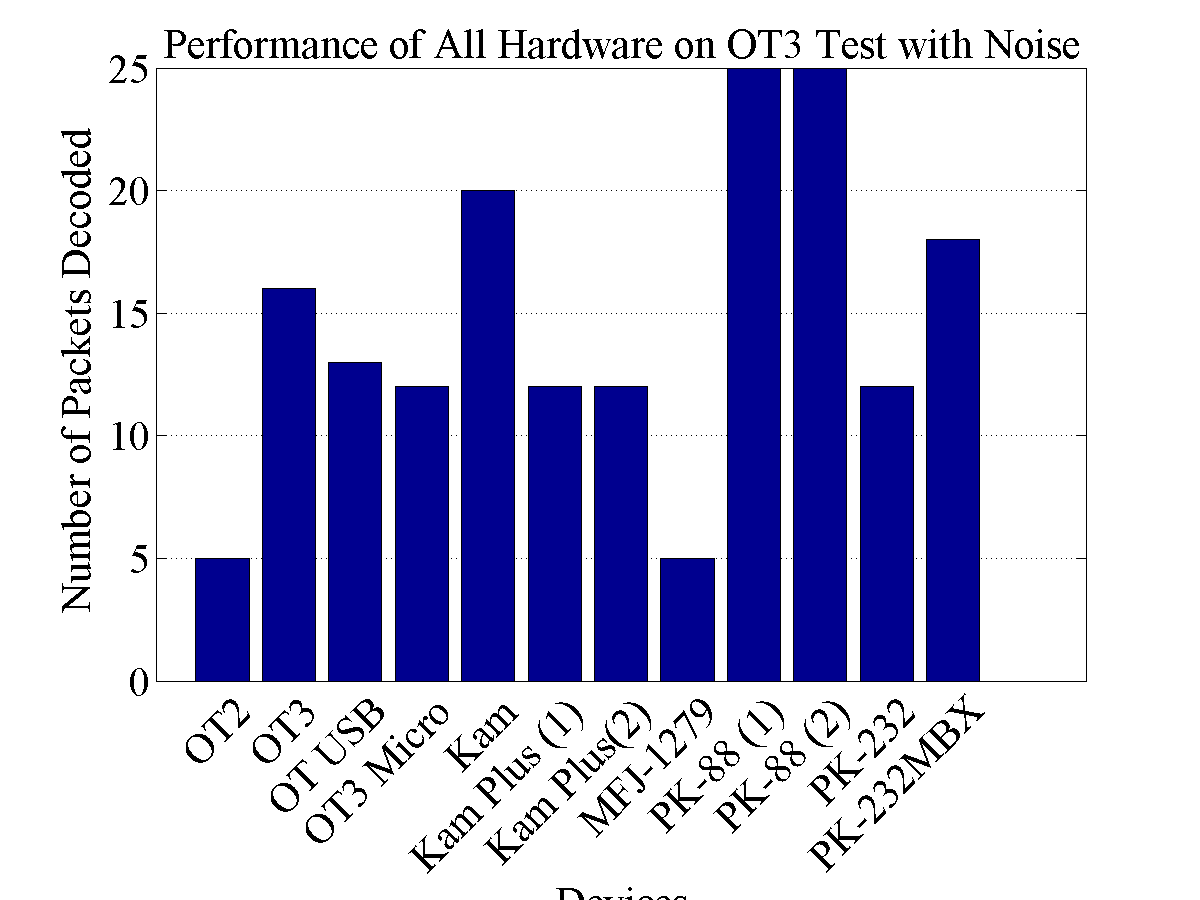
\includegraphics[width=0.75\linewidth]{images/PerformanceofAllHardwareonOT3TestwithNoise.png} 
	\caption{Number of packets successfully decoded for all tested hardware on Open Tracker 3 test file with noise.}
   \label{allHardwareOT3Noise}
\end{figure}

The next two files are the ones that were used most extensively in the testing for comparison and tuning. Primarily the first which is just a recording of traffic off the air. They are Track 1 and 2 from the APRS CD mentioned in the Demodulator Benchmarking Chapter. The results from Track 1 are in Figure \ref{allHardwareTrack1} and Track 2 in Figure \ref{allHardwareTrack2}. The top three of the hardware on Track 1 was the PK-88 (2) with 1007 packets decoded, the Kam with 988 Packets, and the Kam Plus (2) with 985 Packets. For Track 2 the top hardware was the Kam Plus (2) with 998, the Kam Plus (1) with 967, and the Kam with 938.

 \begin{figure}
  \centering
	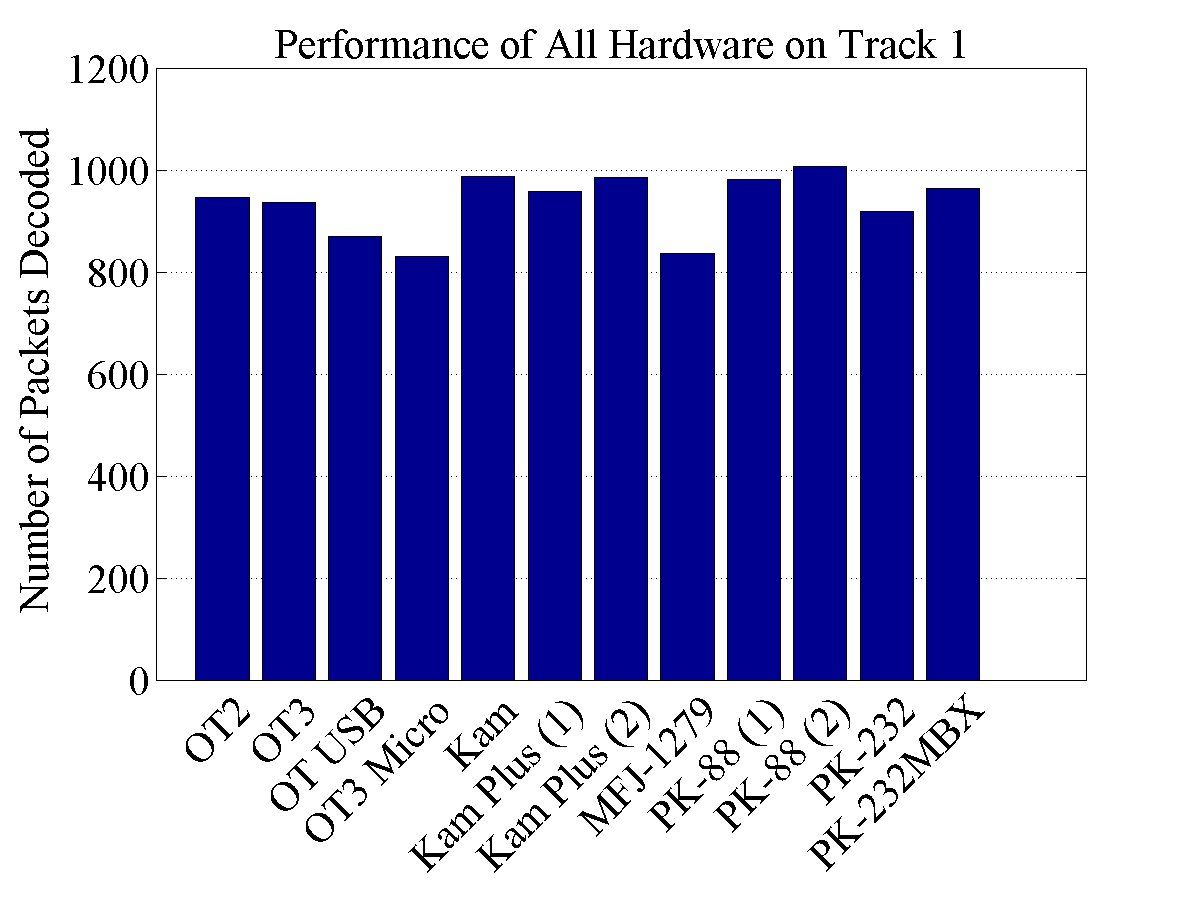
\includegraphics[width=0.75\linewidth]{images/PerformanceofAllHardwareonTrack1.png} 
	\caption{Number of packets successfully decoded for all tested hardware on Open Tracker 3 test file with noise.}
   \label{allHardwareTrack1}
\end{figure}

 \begin{figure}
  \centering
	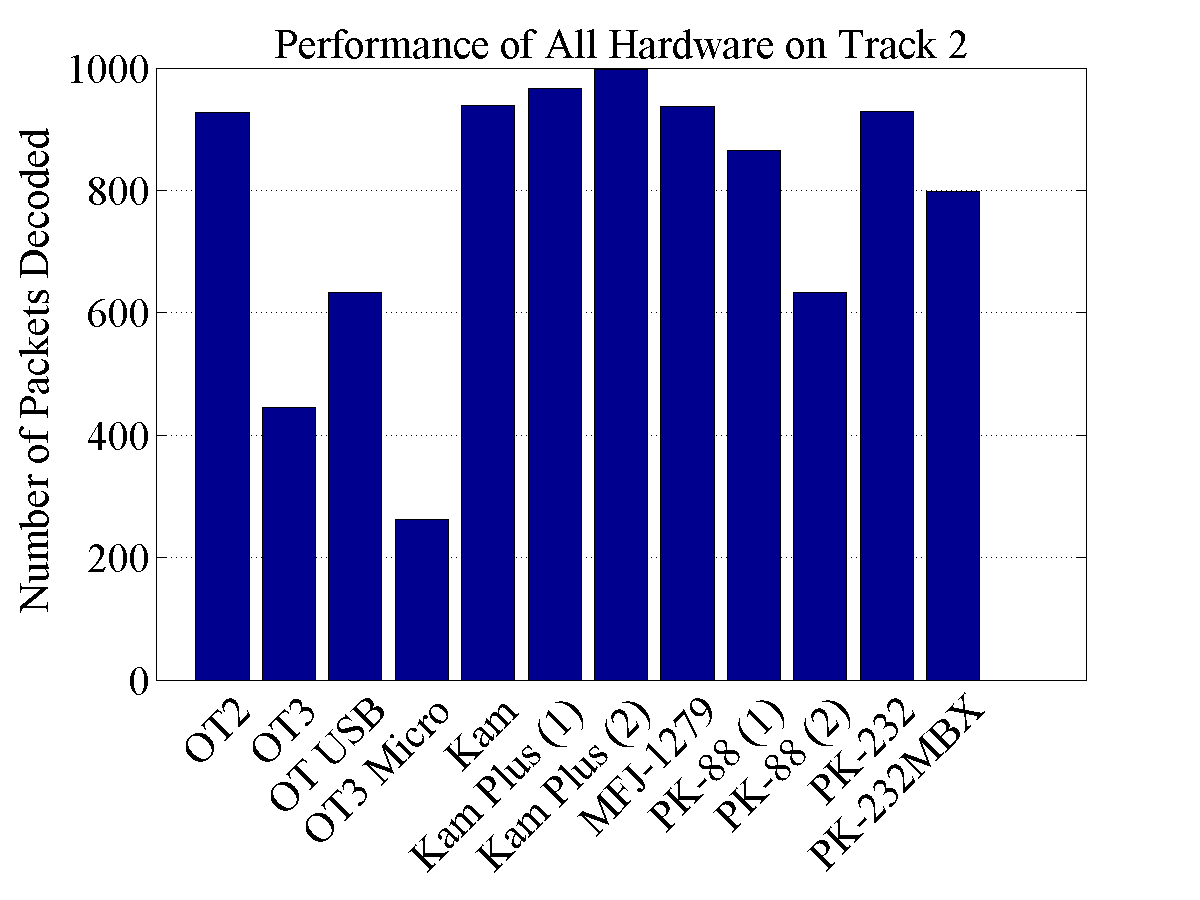
\includegraphics[width=0.75\linewidth]{images/PerformanceofAllHardwareonTrack2.png} 
	\caption{Number of packets successfully decoded for all tested hardware on Open Tracker 3 test file with noise.}
   \label{allHardwareTrack2}
\end{figure}

Using these results the best numbers for the hardware were 40 packets decoded from the Open Track 3 test, 200 from the javAX25 generated file, 25 from the Open Tracer 3 test with added noise, 1007 from Track 1 of the LA test suite, and 998 from Track 2. These best results can be used as a comparison for the software.

\section{Software Results}
In this section the number of packets that each of the demodulators in the javAX25 package was able to decode will be presented. This will include the correlation approach that was already implemented before the start of this research as well as all of the new algorithms that were outlined in the previous chapter on Implementation. However, before getting the results of javaAX25 there is one more data set to be introduced which is the results from another software based demodulation from AGW Packet Engine. Using this software 40 packets decoded from the Open Track 3 test, 200 from the javAX25 generated file, 21 from the Open Tracer 3 test with added noise, 967 from Track 1 of the LA test suite, and 497 from Track 2. The results from javAX25 end up being on par with these results as well as those of the hardware.

With a total of 13 algorithms implemented, some did well and others not at all, so as in the section on hardware results, all of the data will be presented and then a focus on those that performed the best will be taken. In the new javAX25 software implementation the filtering was moved from its original location of being on a per demodulator level basis to a central location that allowed each of the algorithms to utilize it. Some of the algorithms ended up relying on it after tuning and others could remain independent. As such, in order to present all of the data each algorithm will not only have a result for each of the 5 test files, but also for each of the three filters used on the data. The three filters used are no filter, a 900-2500Hz bandpass filter, and the same bandpass with a 6dB attenuation of 1200Hz tones to combat the signals that were not emphasized when transmitted but were deemphasized when received. For instance for the Zero Crossing demodulator there will be three values for the Open Tracker 3 Test file, on at each filtering, and there will continue to be a result value at each filtering for the remaining 4 test files.

Now for the data. On the far left of all the plots will be the correlation data which was the current algorithm that it was the goal of this to beat. The performance of no filter on the Open Tracker 3 Test can be seen in Figure \ref{OT3FiltNo}, Figure \ref{OT3Filt0} is with the bandpass filter, and the emphasizing filter results in Figure \ref{OT3Filt6}. From this data from the Open Tracker 3 test looking at the data for the generated 200 test should look familiar aside from the peak demodulator which was always troublesome other than on this file. The Generated 200 Test file is the only file that the peak demodulator performed comperably. The unfiltered data from this test is in Figure \ref{Gen200FiltNo}, the bandpass data in Figure \ref{Gen200Filt0}, and the results of emphasizing the signal in Figure \ref{Gen200Filt6}.

\begin{figure}
  \centering
	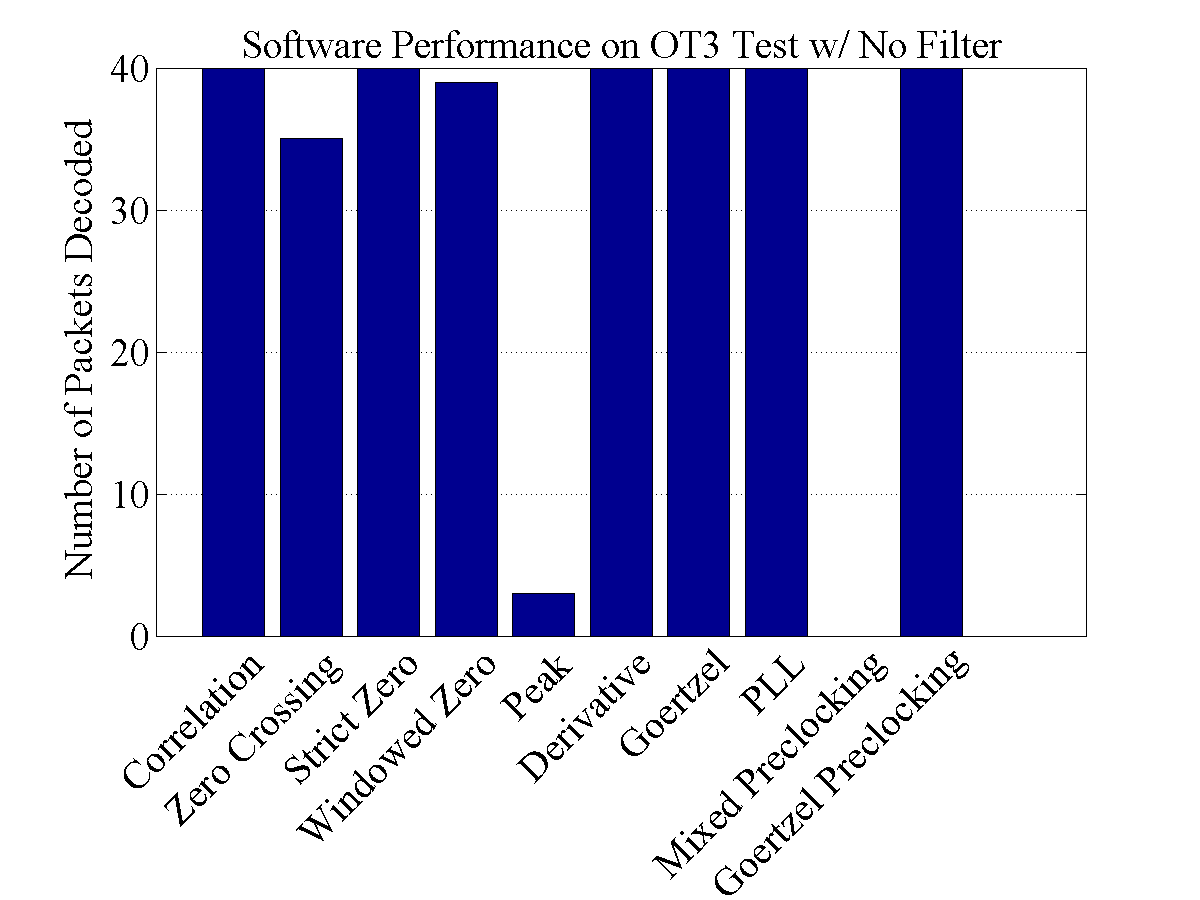
\includegraphics[width=0.75\linewidth]{images/SoftwarePerformanceonOT3TestwNoFilter.png} 
	\caption{Software performance on the raw signal from Open Tracker 3 Test.}
   \label{OT3FiltNo}
\end{figure}
\begin{figure}
  \centering
	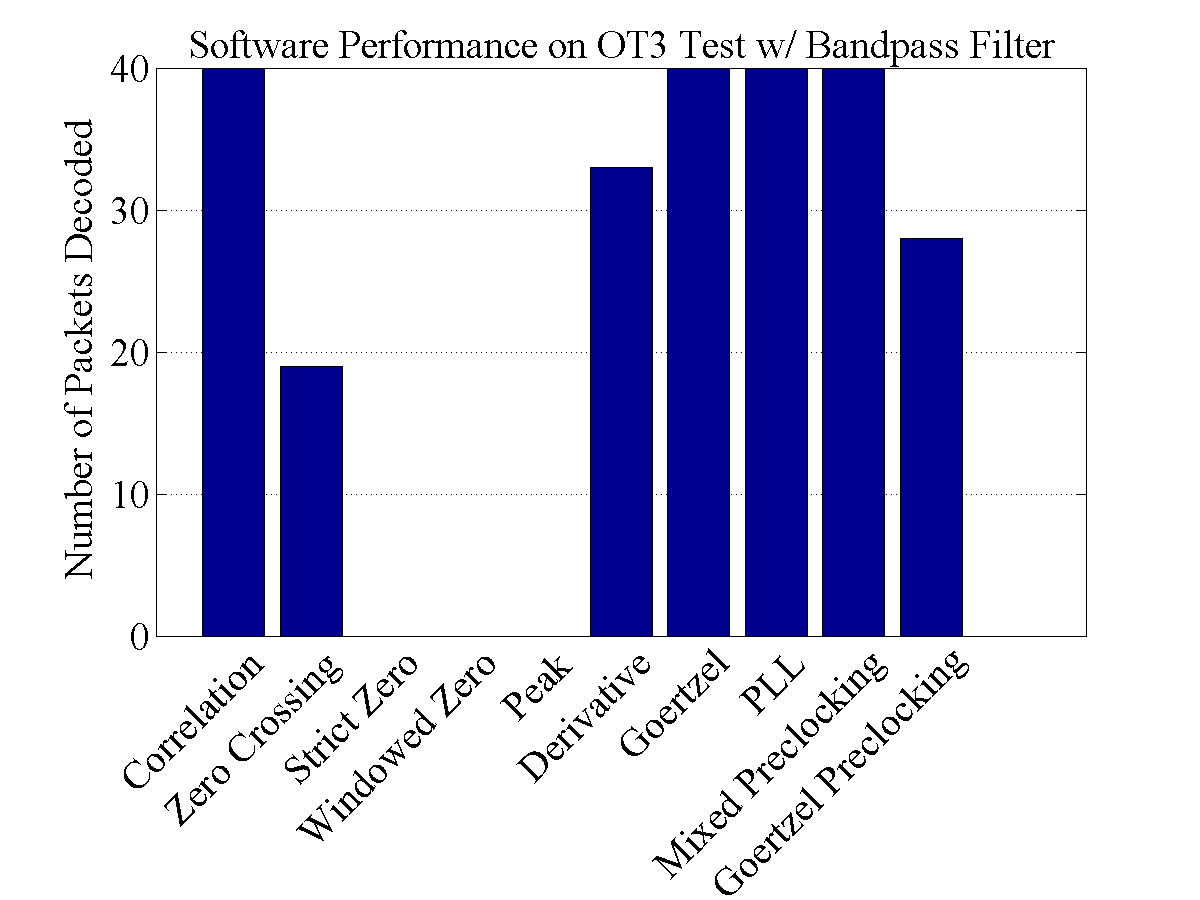
\includegraphics[width=0.75\linewidth]{images/SoftwarePerformanceonOT3TestwBandpassFilter.png} 
	\caption{Software performance with a bandpass filter on Open Tracker 3 Test.}
   \label{OT3Filt0}
\end{figure}
\begin{figure}
  \centering
	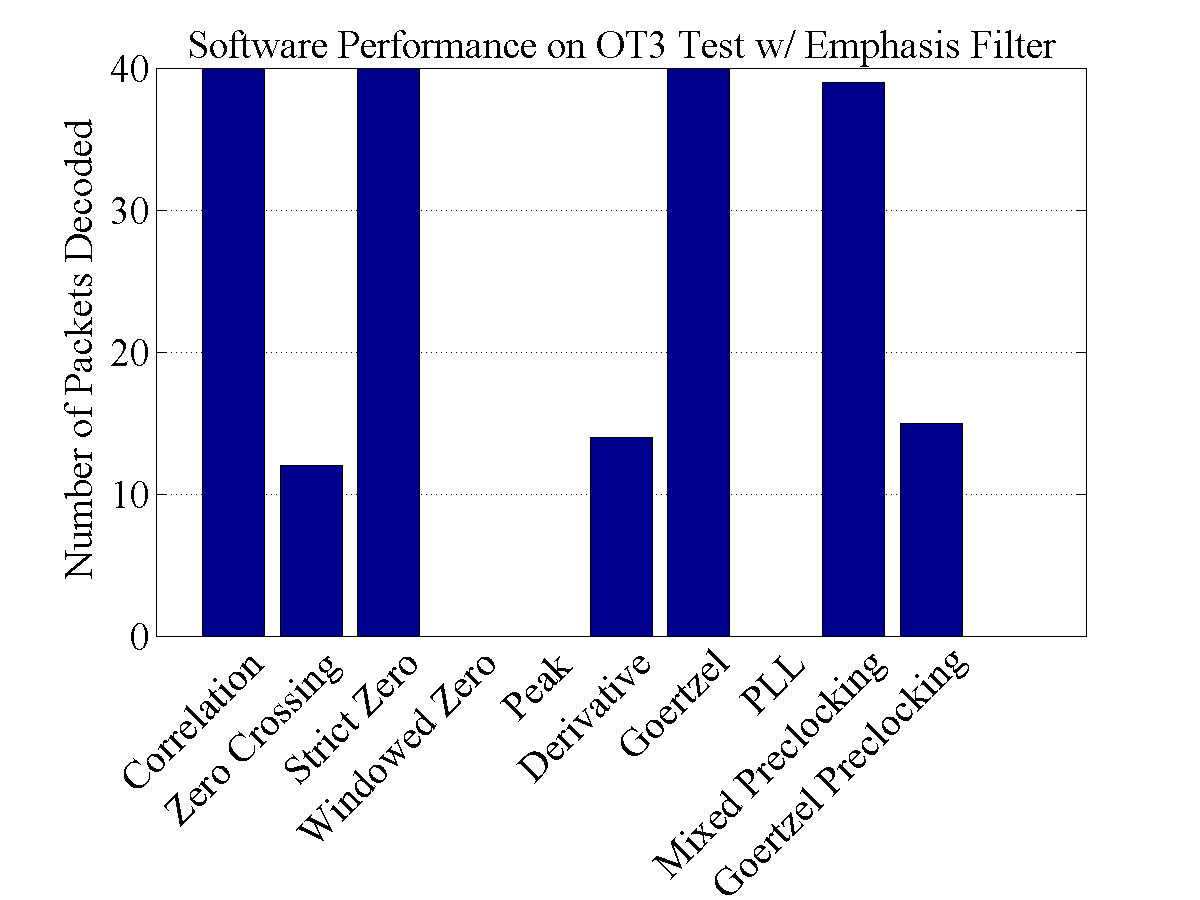
\includegraphics[width=0.75\linewidth]{images/SoftwarePerformanceonOT3TestwEmphasisFilter.png} 
	\caption{Software performance with an emphasis filter on Open Tracker 3 Test.}
   \label{OT3Filt6}
\end{figure}
\begin{figure}
  \centering
	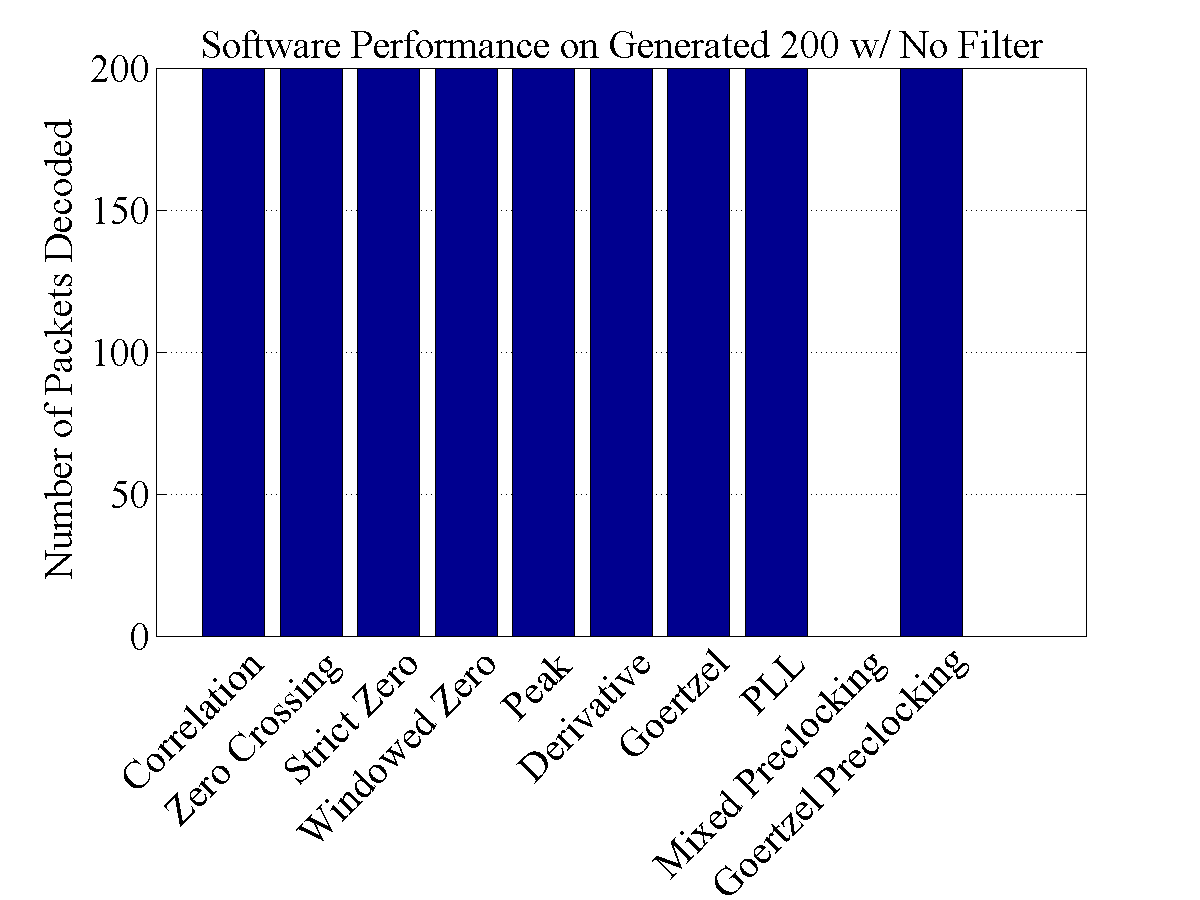
\includegraphics[width=0.75\linewidth]{images/SoftwarePerformanceonGenerated200wNoFilter.png} 
	\caption{Software performance on the raw signal from Open Tracker 3 Test.}
   \label{Gen200FiltNo}
\end{figure}
\begin{figure}
  \centering
	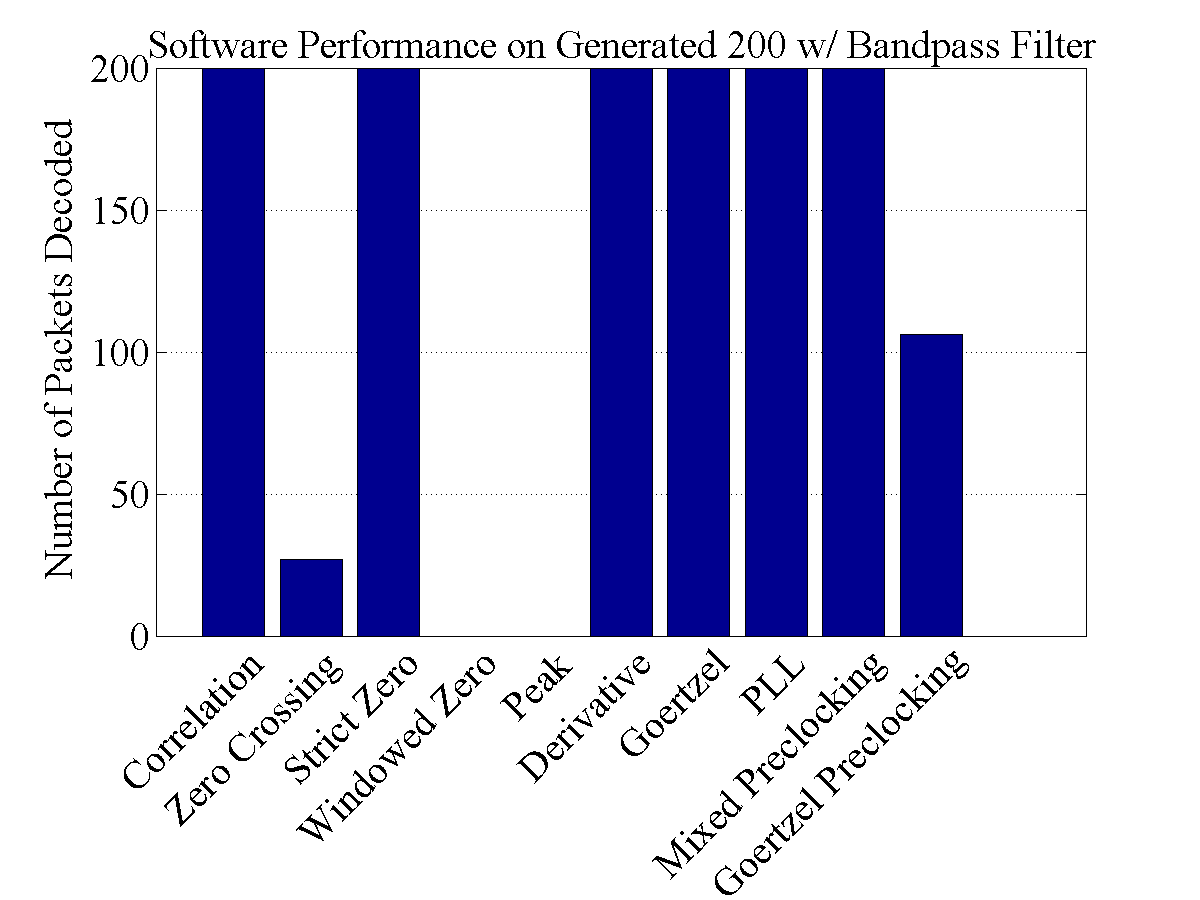
\includegraphics[width=0.75\linewidth]{images/SoftwarePerformanceonGenerated200wBandpassFilter.png} 
	\caption{Software performance with a bandpass filter on Open Tracker 3 Test.}
   \label{Gen200Filt0}
\end{figure}
\begin{figure}
  \centering
	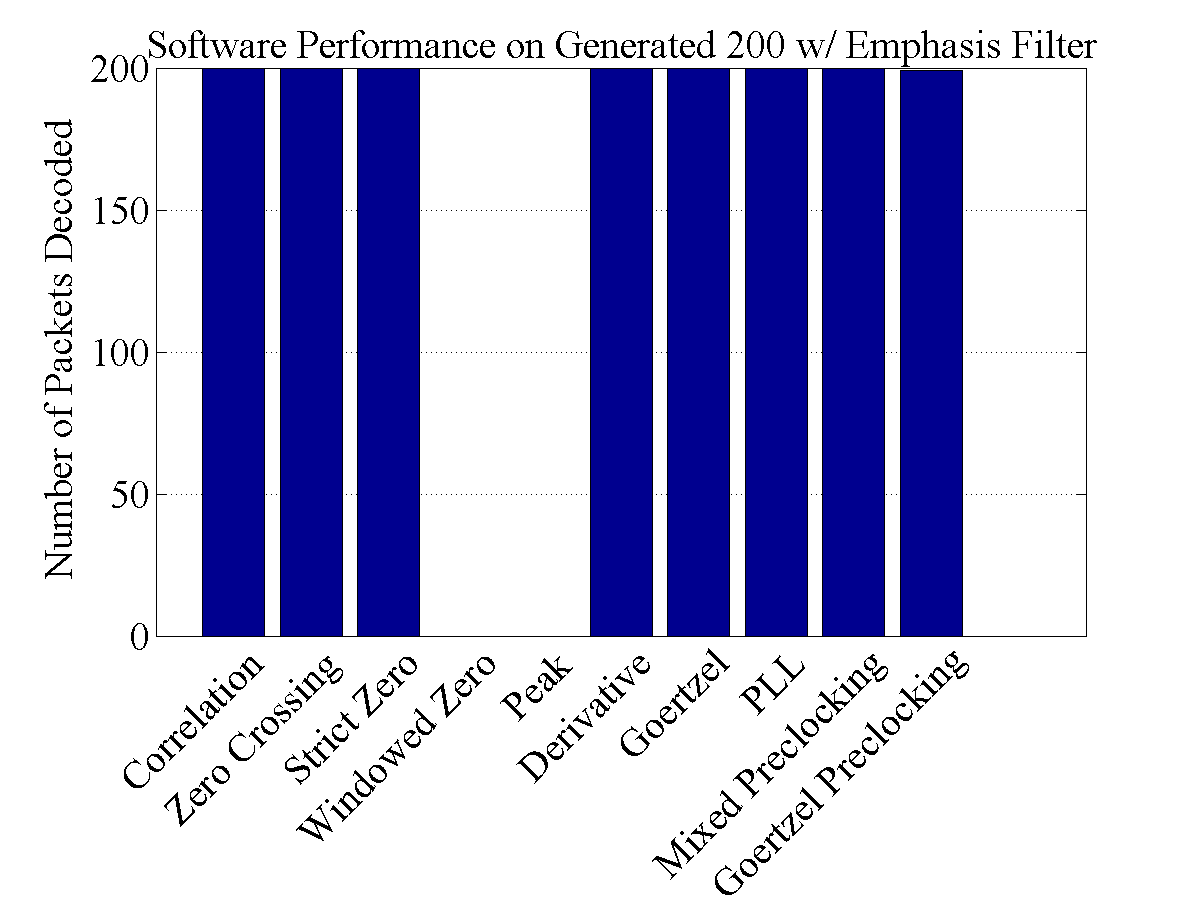
\includegraphics[width=0.75\linewidth]{images/SoftwarePerformanceonGenerated200wEmphasisFilter.png} 
	\caption{Software performance with an emphasis filter on Open Tracker 3 Test.}
   \label{Gen200Filt6}
\end{figure}

\subsection{Hardware and Software Comparisons}

